% Indicate the main file. Must go at the beginning of the file.
% !TEX root = ../main.tex

%----------------------------------------------------------------------------------------
% CHAPTER 2
%----------------------------------------------------------------------------------------
\chapter{Theoretical Background} % Main chapter title
\label{Chapter2} % For referencing the chapter elsewhere, use \ref{Chapter1}
In this chapter, the relevant literature and background information is discussed.  
\section{Cellular Automata}
\subsection{A Brief History}

Cellular Automata are fascinating computational models, which typically have very simple rules that result in complicated behavior. They were first introduced by John Von Neuman \cite{sarkar2000brief} as models for self-replicating organisms. Since then they have found relevance in an extremely wide variety of fields but mainly used in modeling biological and physical systems. \\
Typically, Cellular Automata are modeled on a discrete 1D or 2D lattice. The most famous Cellular Automata are John Conway's Game of Life (GOL) and Steven Wolfram's Elemetary Cellular Automata, the former of which will be discussed in the below section.
From here on 'Cellular Automata' and 'Cellular Automaton' will be referred to as CA.
\subsection{What is a CA?}

CA are some of the simplest computational models that exist. They consist of a discrete lattice or grid of cells (Typically these manifolds are 1D or 2D but can be $d$ dimensional). Each cell has a discrete state (or set of states). The most common of which, are binary states like in the case of Elementary CA and GOL \footnote{It is important to note, though, that variations of this exist and a lot of research has been done in the continuous state domain. A famous example of this within the CA community is Lenia: Smooth life \cite{chan2018lenia}. The reason for this note is CA used for flood modeling as well as some other systems utilize this continuous state system}. Probably the most important aspect of CA systems are their local update rules'. In order for a cell to be updated, the cell considers the states of itself, as well as the states of its neighbors, and based on some rule, the cell updates. In classical CA, cells update synchronously based on some global clock \footnote{This feature of classical CA also has variation, like in the case of stochastic CA \cite{fates2013stochastic}, where cells update asynchronously.}. Based on these features, very simple rules can result in extremely complex behaviour. \\
To help build intuition about CA and its associated notation, I will discuss John Conway's Game Of Life. Game of Life will be mentioned a lot in this thesis because it is a simple example and widely known CA.

\subsection{Mathematical Description of CA Using Game Of Life as an example}

\subsubsection*{Defining Game Of Life}
The following are the general rules written in natural language and in the subsequent section we will demonstrate the notation used for such as system.

\begin{enumerate}[align=left]
	\item[Grid:] The Game of Life is represented as a two-dimensional grid of cells. Each cell can be either alive or dead, usually represented by binary values: 1 for alive and 0 for dead. The grid is typically depicted as a matrix-like structure.
	\item[Neighbourhood:] Each cell in the Game of Life has a neighborhood consisting of its eight adjacent cells. This neighborhood is known as the Moore neighborhood. The state of a cell is influenced by the states of its neighboring cells according to the game's rules.
	\item[States:] In the Game of Life, each cell can be in one of two states: alive (1) or dead (0). This binary representation simplifies the rules and allows for the emergence of interesting patterns and behaviors.
	\item[Local Update Rule:] The evolution of the Game of Life is determined by a set of rules that dictate how cells change their states over time. These rules are applied simultaneously to all cells in the grid. The rules of the Game of Life are as follows:
	\begin{enumerate}
		\item Any live cell with fewer than two live neighbors dies, as if by under population.
		\item Any live cell with two or three live neighbors survives to the next generation.
		\item Any live cell with more than three live neighbors dies, as if by overpopulation.
		\item Any dead cell with exactly three live neighbors becomes alive, as if by reproduction.
	\end{enumerate}
\end{enumerate}

By applying these rules iteratively, the Game of Life evolves and creates various patterns, including static configurations, oscillators, and spaceships that move across the grid. The simplicity of the rules gives rise to complex and intriguing dynamics within the cellular automaton known as the Game of Life.

\subsubsection*{Representing GOL Mathematically}

 An arbitrary CA is typically represented as a 4-tuple, with time, $T$, left out:
\begin{equation}
	A = (L, S, N, f)
\end{equation}

where:

\begin{align*}
	A &  \text{ is the CA} \\
	L &  \text{ is the } d \text{-dimensional lattice} \\
	S &  \text{ is the set of possible states} \\
	N &  \text{ is the neighbourhood} \\
	f &  \text{ is the local update rule}
\end{align*}

\textbf{need to add the math here}
\subsection{Why are they useful?}
In the above section, although beautiful and impressive, the examples are not practival. But the same motivation and methods can be extrapolated to model physical or biological systems. Especially many differentiable equations that can be descritized in time and space can be modeled using CA. Many examples have been demonstrated over the years. In the following \ref{Chapter3}, the CADDIE2D model is discussed in detail. But other examples include: particle simulation, chemical reactions, fire modeling, human and animal dynamics to name a few. [must find references for this.]

\section{Deep Learning}
\subsection{What Is Deep Learning}

Deep learning is a subset of techniques within a class of algorithms called Machine Learning (ML). In general, ML algorithms power increasingly more of our day to day lives \cite{lecun2015deep}. From auto-correct on word processors, to search engines, to recommendation systems, and even self-driving cars. The list goes on. \\

Deep learning is derived from simple neural networks. The consist of nodes and edges. They tend to look like this:

% Input layer neurons'number
\newcommand{\inputnum}{3} 

% Hidden layer neurons'number
\newcommand{\hiddennum}{5}  

% Output layer neurons'number
\newcommand{\outputnum}{2} 

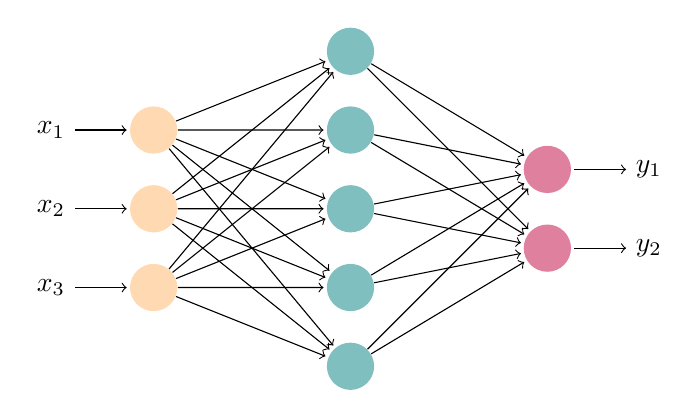
\begin{tikzpicture}

	% Input Layer
	\foreach \i in {1,...,\inputnum}
	{
		\node[circle, 
		minimum size = 6mm,
		fill=orange!30] (Input-\i) at (0,-\i) {};
	}
	
	% Hidden Layer
	\foreach \i in {1,...,\hiddennum}
	{
		\node[circle, 
		minimum size = 6mm,
		fill=teal!50,
		yshift=(\hiddennum-\inputnum)*5 mm
		] (Hidden-\i) at (2.5,-\i) {};
	}
	
	% Output Layer
	\foreach \i in {1,...,\outputnum}
	{
		\node[circle, 
		minimum size = 6mm,
		fill=purple!50,
		yshift=(\outputnum-\inputnum)*5 mm
		] (Output-\i) at (5,-\i) {};
	}
	
	% Connect neurons In-Hidden
	\foreach \i in {1,...,\inputnum}
	{
		\foreach \j in {1,...,\hiddennum}
		{
			\draw[->, shorten >=1pt] (Input-\i) -- (Hidden-\j);   
		}
	}
	
	% Connect neurons Hidden-Out
	\foreach \i in {1,...,\hiddennum}
	{
		\foreach \j in {1,...,\outputnum}
		{
			\draw[->, shorten >=1pt] (Hidden-\i) -- (Output-\j);
		}
	}
	
	% Inputs
	\foreach \i in {1,...,\inputnum}
	{            
		\draw[<-, shorten <=1pt] (Input-\i) -- ++(-1,0)
		node[left]{$x_{\i}$};
	}
	
	% Outputs
	\foreach \i in {1,...,\outputnum}
	{            
		\draw[->, shorten <=1pt] (Output-\i) -- ++(1,0)
		node[right]{$y_{\i}$};
	}
	
\end{tikzpicture}

The main difference between classical ML and DL is the former tends to require large amounts of domain knowledge and heavy feature engineering. "The best deep learning models require no domain knowledge" (Personal Communication, Edan need to find surname). 
Artificial Neural Networks can learn the feature importance. \\

maybe too far??


Things to talk about:
\begin{itemize}
	\item What is classical ML
	\item What is the problem with classical approaches
	\item What is deep learning and how does it improve on classical ML
	\item Briefly backprop and optimizers and loss functions
	\item I guess CNN's will go in here too
	\item general evaluation of model and importance of generalization
\end{itemize}
\subsection{The Tensorflow Framework}
\begin{itemize}
	\item Quickly mention the framework and how it is an extremely popular and fast library in python for building deep learning models. It mainly works through the use of tensors (d-dimensional matrix). It has many useful functions for creating models, performing back propogation. There are two other frameworks that people generally use: JaX and Pytorch. The descision for which to use is relatively arbitrary and is typcially based on what a company / researcher has used in the past.
\end{itemize}
\subsection{Optimizers for backpropogation}
\subsection{Common loss functions for regression tasks}
I create this subsection because I think this needs to be carefully considered. For growing images, L2
loss is clearly the best option to reproduce images / learning to grow them. However, depending on
the application of these models the loss function needs to be carefully considered and there are many
to choose from. An example of this is from the paper [3, Self-Organizing Textures] where they use a
L2 loss of gram-matrices by using the raw activations of VGG (Visual Geometry Group Net).
Here we can also look into applying physical constraints to the model, for e.g. adhering to energy
/ mass conservation.
\subsection{Convolutional Neural Network}

A Convolutional Neural Network (CNN) is a type of Artificial Neural Network (ANN) that is commonly used in image and video recognition, natural language processing, and other tasks that involve processing input data with a grid-like structure.

The key characteristic of a CNN is the use of convolutional layers, which apply a set of filters to the input data to extract relevant features for the task at hand. The filters are typically small in size and designed to detect simple patterns, such as edges or corners. The output of the convolutional layer then goes through a non-linear activation function, such as the rectified linear unit (ReLU), to introduce non-linearity into the network.

In addition to convolutional layers, a CNN may also include other types of layers such as pooling layers, which reduce the spatial dimensions of the input data by selecting the maximum or average value from a set of neighboring pixels, and fully connected layers, which connect every neuron in one layer to every neuron in the next layer.

CNNs have achieved state-of-the-art performance on many computer vision tasks, such as image classification, object detection, and segmentation, and are widely used in industry and academia.

\section{The Relationship Between CA and CNN}
\subsection{CNN as a CA}
As it turns out, CNN's are extremely similar. Cellular automata (CA) and convolutional neural networks (CNN) are both types of mathematical models that can be used to process and analyze data with a grid-like structure, such as images or time series data. \cite{PhysRevE.100.032402}

Both models operate by processing the input data in a local and hierarchical manner. In a CA, the state of each cell is updated based on the states of its neighboring cells, while in a CNN, filters are applied to local patches of the input data to extract relevant features. However, one can think of a neighbourhood as a $NxM$ kernel or filter. In fact, by utilizing a cleverly constructed kernel and activation function, one can model many CA. A simple example of this would be game of life represented as a convolution. \\

A convolution is defined as: \\

\begin{equation*}
	g(x,y) = \omega f(x, y)
\end{equation*}
Where:
\begin{align*}
	f &: \text{is the function to be convolved} \\
	\omega &: \text{is the kernel}  \\
	g &: \text{is the convolution} 
\end{align*} 

We can create a kernel, $\omega$, which looks like: \\

$
\begin{bmatrix}
	1 & 1 & 1 \\
	1 & 9 & 1 \\
	1 & 1 & 1
\end{bmatrix}
$
\\

And then add an activation function, $\sigma$: \\ \\

%% I should really add more mathematics here
$
\sigma(x, y) = \begin{cases}
	1, & \text{if } g(x, y) = 3 | 11 | 12 \\
	0, & \text{otherwise}
\end{cases}
$
\\ \\


It turns out that CNN's can learn the rules of arbitrary CA's, for example game of life, and it doesn't need a particularly deep architecture to do so. it does this by essentially learning the kernel / filter weights that needs to be applied. To use a CNN as a CA, you essentially turn the CA into a binary classification problem to predict the state of each cell.

\subsection{Neural Cellular Automata}

Now that we have some basic foundational knowledge we can move on to the real NCA (or differentiable, self-organizing systems). As discussed in the section above, a CNN can be seen as a type of CA, but utilizing a continuous state-space instead of a discrete one (as well as an arbitrary number of hidden states / channels). As described in the growing NCA paper \citetitle{growing_nca}, this model can be thought of as a “Recurrent Residual Convolutional Network with ‘per-pixel’ Dropout”. The 'per-pixel dropout' refers to the stochastic updating of cells. We start from a single black pixel in the center of a blank image and run the model on it for a certain number of steps where the output of the model becomes the new input. Then compare the final result of this model with the target image we are training the model. We then perform a per-pixel difference loss function (L2 loss). Then based on this loss we use ADAM optimizer to back-propagate through time to adjust the weights of the model until the model learns to 'grow' the target image from a seed state.a seed state.
